\documentclass{ra2003}
\usepackage{amsfonts}
\usepackage{amsmath}
\theme{3a}
\isproject{YES} % \isproject{OUI} works also
\projet{exemple}{Miaou}{Math�matiques et Informatique de l'Automatique et de l'Optimisation pour l'Utilisateur}
\UR{\URSophia\URFuturs}

\def\CC{{\mathbb C}}
\newcommand{\etc}{etc}
\def\corresp{manager}

\declaretopic{abc}{Topic abc}
\declaretopic{def}{Topic def}

\begin{document}


\begin{filecontents+}{exemple2003.bib}
@InProceedings{tralics-eurotex,
  author = 	 {Jos� Grimm},
  title = 	 {Tralics, a {\LaTeX} to XML Translator},
  booktitle = 	 {Proceedings of Eurotex},
  year = 	 2003
}

@Misc{brevet,
  author =	 {{European patent No. 03292257.7-}},
  note =	 {Title: ``wavelength converter''. Applicant/proprietor: Alcatel. Inventors: B. Lavigne, O. Leclerc, J.-P. Moncelet, A. Bombrun, F. Seyfert, J.-B. Pomet},
  month =	 sep,
  year =	 2003,
  howpublished = {European patent office}
}

@Article{blpprep,
  author =     {L. Baratchart and J. Grimm and J. Leblond and
                  J. R. Partington},
  title =      {Approximation and interpolation in $H^2$: Toeplitz
                  operators, recovery problems and error bounds},
  journal =    {Integral Equations and Operator Theory},
 year =        2003,
  volume =     45,
pages={269--299}
}
\end{filecontents+}

\begin{filecontents+}{exemple_refer2003.bib}
@Article{BO1,
  author =	 {L. Baratchart and M. Olivi},
  title =	 {Critical points and error rank in best $H^2$ matrix rational
                  approximation of fixed McMillan degree},
  journal =	 {Constructive Approximation},
  volume =	 14,
  year =	 1998,
  pages =	 {273-300}
}

@Article{lo,
  author =	 {J. Leblond and M. Olivi},
  title =	 {Weighted {$H^2$} approximation of transfer functions},
  journal =	 "Math. of Control, Signals \& Systems (MCSS)",
  year =	 1998,
  volume =	 11,
  pages =	 {28-39},
}
\end{filecontents+}

\begin{filecontents+}{exemple_foot2003.bib}
@Article{lswprep,
  author =       {J. Leblond and E.B. Saff and F. Wielonsky},
  title =        {Weighted {$H_2$} rational approximation and consistency
                  properties},
  journal =      {Numerische Mathematik},
  volume = 	 90,
  number = 	 3,
  pages = 	 {521-554},
xxurl= {http://dx.doi.org/10.1007/s002110100281},
doi={10.1007/s002110100281},
year =       2002
}

@article{partII,
  author =	 {L. Baratchart and J. Leblond},
  title =	 {Hardy approximation to {$L^p$} functions on subsets of the
                  circle with $1 \leq p < \infty$},
  journal =	 {Constructive Approximation},
  year =	 1998,
  volume =	 14,
  pages =	 {41-56}
}

\end{filecontents+}



\maketitle
\nocite{*}

\begin{module}{composition}{en-tete}{}

\begin{catperso}{Head of project team}
\pers{Laurent}{Baratchart}[DR INRIA]
\end{catperso}

\begin{catperso}{Vice-head of project team}
\pers{Juliette}{Leblond}[CR INRIA]
\end{catperso}

\begin{catperso}{Administrative assistant}
\pers{France}{Limouzis}[AI INRIA, partial time in the project]
\end{catperso}

\begin{catperso}{Staff member}
\pers{Jos�}{Grimm}[CR INRIA]
\end{catperso}

\begin{catperso}{Ph. D. Students}
\pers{David}{Avanessoff}[Fellow, INRIA]
\pers{Alex}{Bombrun}[Since November, 1st]
\pers{Moncef}{Mahjoub}[Co-advised, ENIT Tunis (in France in February, March, October, November)]
\end{catperso}
\end{module}

\begin{module}{presentation}{presentation}{}
\begin{moreinfo}
The project was terminated June the 30th, 2003. 
A proposal for a new project named APICS has been submitted to the steering
comittee of Inria Sophia Antipolis.
\end{moreinfo}

The Team develops effective methods for modelling, identification and control
of dynamical systems.

\subsubsection*{Research Themes}
\begin{itemize}
\item Meromorphic and rational approximation in the complex domain,
  application to identification of transfer functions  and matrices as well as
  singularity detection for 2-D Laplace operators. Development of 
%the hyperion
  software for frequency domain identification and synthesis of transfer
  matrices.  
\item Control and structure of non-linear systems: continuous stabilization,
  non-linear transformations (linearization, classification). 
\end{itemize}

\subsubsection*{International and industrial partners}

\begin{itemize}
\item Industrial collaborations with Alcatel-Space, \etc
\item Exchanges with CWI CNR (Italy), \etc
\item The project is involved in a NATO Collaborative Linkage Grant \etc
\end{itemize}
\end{module}


\begin{module}[def]{fondements}{identif}{Identification and deconvolution}
Let us first introduce  the subject of Identification in some generality.

Abstracting in the form 
of mathematical equations the behavior of a phenomenon is
a step called \emph{modeling}. It typically serves two purposes: the first
is to describe the phenomenon with minimal complexity for some specific 
purpose,
the second is to \emph{predict} its outcome. \etc


\subsubsection{Analytic approximation of incomplete boundary data}
\label{dida-mero}
\label{filtrescnes}
\label{didactique-approx-rat-mat}
\begin{participants}
\pers{Laurent}{Baratchart},
\pers{Jos�}{Grimm},
\pers{Birgit}{Jacob}[University of Leeds (GB)],
\pers{Juliette}{Leblond},
\pers{Jean-Paul}{Marmorat}[CMA, �cole des Mines],
\pers{Jonathan}{Partington},
\pers{Fabien}{Seyfert}
\end{participants}

\begin{motscle}
meromorphic approximation, frequency-domain identification,
extremal problems 
\end{motscle}

\etc, so that a prototypical Problem is:

{\sl ($P$)~~Let $p \geq 1$, $N \geq 0$, $K$ be an arc of the unit circle $T$, 
  $f \in L^p(K)$, $\psi \in L^p(T \setminus K)$ and $M>0$;
  find a function  $g \in H^p + R_N$ such that 
  $\|g - \psi\|_{L^p(T \setminus K)} \leq M$ and such that $g - f$ 
  is of minimal norm in  $L^p(K)$ under this constraint.}

Problem ($P$) is an extension to the meromorphic case, and to incomplete data,
of classical analytic extremal problems (obtained
by setting $K=T$ and $N=0$), that generically go under the name
\textit{bounded extremal problems}. 
These have been introduced and intensively studied by the Team, 
\cite{blpprep} and ~\footcite{partII}. 

\subsubsection{Scalar rational approximation}
\label{didactique-approx-rat-scal}
\begin{participants}
\pers{Laurent}{Baratchart},
\pers{Reinhold}{K�stner},
\pers{Juliette}{Leblond},
\pers{Martine}{Olivi},
\pers{Edward}{Saff},
\pers{Herbert}{Stahl},
\pers{Franck}{Wielonsky}
\end{participants}

\begin{motscle}
rational approximation, critical point, orthogonal polynomials
\end{motscle}
\etc.
\begin{equation}
\label{crit}
\left\|f - \frac{p_m}{q_n} \right\|_{L^2(d \mu)} 
\end{equation}
where, by definition, 
\[
\|g\|_{L^2(d \mu)}^2=\frac{1}{2\pi} \int_{-\pi}^{\pi}|g(e^{i\theta})|^2
d\mu(\theta),
\]

\etc

If one introduces now as a new variable the rational matrix $R$ defined by
\[
R=\left(\begin{array}{cc}
L            &  H \\
0            &   I_m
\end{array} \right)^{-1}
\]
and if $T$ stands for the first block-row, 
normalizing the variance of the noise to be identity, the maximum likelihood
estimator  is asymptotically equivalent, when the sample size increases, 
to the minimization of
\begin{equation}
\label{defLL}
\|T\|_{\Lambda}^2={\bf Tr}\left\{\frac{1}{2\pi}
\int_{0}^{2\pi}T(e^{i\theta})\,
d\Lambda(\theta)\,T^*(e^{i\theta})\right\},
\end{equation}
where $\Lambda$  is the spectral measure  of the process $(y~u)^t$ 
(which positive and matrix-valued)
and where  ${\bf Tr}$ indicates the trace. 

\subsubsection{Continuous stabilization}
Stabilization by continuous state feedback \etc

\paragraph{Periodic stabilisation of non-linear systems.}
It is known that \etc

\paragraph{Control Lyapunov functions.}
Lyapunov functions  are \etc
\end{module}

\begin{module}{domaine}{chapeau}{}
The activity of the team focuses on two bottom lines, namely \etc
\end{module}


\begin{module}{}{dom-fissures}{Geometric inverse problems 
for the Laplacian}
\begin{participants}
\pers{Laurent}{Baratchart}
\end{participants}

\begin{motscle}   % non destructive
inverse problem, Laplace equation, non destructive control, tomography
\end{motscle}

Localizing cracks, \etc
\end{module}


\begin{module}{domaine}{resonn}{Identification and design of resonant systems}
\begin{motscle}
telecommunications, multiplexing, filtering device, hyperfrequency, surface waves
\end{motscle}
Some text.
\end{module}

\begin{module}[abc]{domaine}{spatial}{mechanics}
\etc
\end{module}


\begin{module}[def]{domaine}{optique}{Non-linear Optics}
\etc
\end{module}


\begin{module}{domaine}{plat}{Transformations and equivalence of non-linear systems}

\begin{participants}
\pers{Laurent}{Baratchart},
\pers{Jean-Baptiste}{Pomet},
\pers{David}{Avanessoff}
\end{participants}

\begin{motscle}
path planning, mobile cybernetics,  identification, {(max,plus) algebra}
\end{motscle}
\etc
\end{module}

\begin{module}{logiciels}{hyperion}{The hyperion software}

\begin{participants}
\pers{Jos�}{Grimm}[\corresp],
\pers{Fabien}{Seyfert},
\pers{Franck}{Wielonsky}
\end{participants}
\etc
\end{module}

\begin{module}{logiciels}{logi-tralics}{The Tralics software}

\begin{participant}
\pers{Jos�}{Grimm}[\corresp]
\end{participant}
\etc. \nocite{tralics-eurotex}
\end{module}

\begin{module}{logiciels}{RARL2}{The RARL2 software}
\begin{participant}
\pers{Jean-Paul}{Marmorat},
\pers{Martine}{Olivi}[\corresp]
\end{participant}

RARL2 (R�alisation interne et Approximation Rationnelle L2) is a software for
rational approximation (see module \ref{didactique-approx-rat-mat}). Its web
page is
\htmladdnormallink{\url{http://www-sop.inria.fr/miaou/RARL2/rarl2.html}}
{http://www-sop.inria.fr/miaou/RARL2/rarl2.html}.
\end{module}

\begin{module}{logiciels}{RGC}{The RGC software}


\begin{participants}
\pers{Fabien}{Seyfert},
\pers{Jean-Paul}{Marmorat}
\end{participants}

The RGC software \etc
\end{module}

\begin{module}{logiciels}{PRESTO-HF}{PRESTO-HF}
\begin{participant}
\pers{Fabien}{Seyfert}
\end{participant}

PRESTO-HF: a toolbox dedicated to lowpass parameter identification for
hyperfrequency filters
\htmladdnormallink{\url{http://www-sop.inria.fr/miaou/Fabien.Seyfert/Presto_web_page/presto_pres.html}}
{http://www-sop.inria.fr/miaou/Fabien.Seyfert/Presto_web_page/presto_pres.html}
\etc

\end{module}

\begin{module}{resultats}{tralics}{Tralics: a Latex to XML Translator}

The main philosophy of Tralics is to have the same parser as \TeX, but the
same semantics as \LaTeX. This means that commands like \verb+\chardef+, 
\verb+\catcode+, \verb+\ifx+, \verb+\expandafter+, \verb+\csname+, etc.,
that are not described in the \LaTeX\ book and not implemented in translators
like latex2html, tth, h�v�a, etc., are recognised by Tralics. This year we
added constructions like \verb=\endlinechar=, \verb=\read=,
\verb=\uppercase=, \verb=\endinput=, which are less used, and a bit tricky. 
Note that a construction like \verb=\ifdim\wd0>0pt\fi= is recognised by the
parser, but there is no way to change the size of the box number zero, so that
the test is always false. 

For more information, see the
\htmladdnormallink{Tralics web page}{http://www-sop.inria.fr/miaou/tralics/}.

\begin{figure}
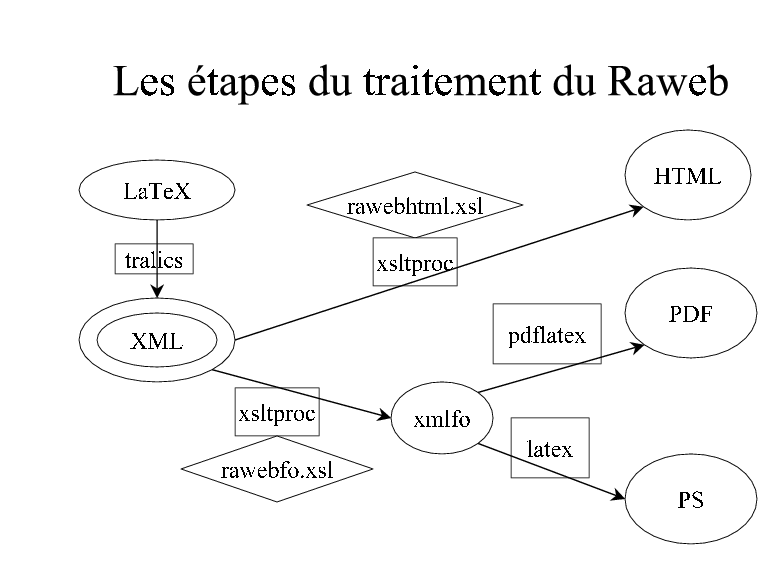
\includegraphics[width=15cm]{xml-route}
\label{xml-route}
\caption{A slide that explains how the raweb operates. Rectangular boxes contain
  tools, diamond-shape boxes are style sheets, and ellipses contain language
  names; the name XML is in a double ellipse, it is the central object. The
  Perl script that handles the math formulas is not shown here;  it uses tools
  borrowed from latex2html.}
\end{figure}

\end{module}

\begin{module}{resultats}{Couplages-Algebrique}{Parametrizations  of matrix-valued lossless functions}
\etc
\end{module}

\begin{module}{resultats}{martine2}{The mathematics of Surface Acoustic Wave filters}
\etc
\end{module}


\begin{module}{resultats}{nat}{Scientific Committees}

L. Baratchart is member of the editorial board of \textit{Computational
Methods in Function Theory}.

\end{module}


\begin{module}[abc]{contrats}{cnes}{Contract ABCD-EFGH-INRIA}

Contract \no 1 03 E 2145% this number is OK

In the framework of a contract that links  ABCD, EFGH and Inria, 
whose objective is \etc the work of Inria has been
\begin{itemize}
\item \etc see module \ref{filtrescnes},
\item \etc  (see module  \moduleref{MIAOU}{resultats}{Couplages-Algebrique}),
\item modeling and \etc, see module \ref{filtrescnes}.
\end{itemize}
In this contract, we promised version 1 of our software to both partners.
This contract has been renewed in 2003.
\end{module}


\begin{module}{contrats}{aspi-c}{Contract Company Somename (Cannes)}

Contract \no 1 01 E 0736.

This contract started in 2001, for three years. 
The objective is \etc
\end{module}

\begin{module}{contrats}{c-marcoussis}{Contract OtherName}

Contract \no 1 02 E 0327.
This was a one year contract, that ended formally in February, 2003.
\begin{description}
\item[Subject.] Objective was \etc
\item[Outcome.] We have contributed to \etc
\end{description}
\end{module}



\begin{module}{international}{nationale}{National Actions}

Together with project-teams Caiman and Odyss�e
(INRIA-Sophia Antipolis, ENPC), the University of Nice (J.A. Dieudonn� lab.), 
CEA, CNRS-LENA (Paris), and a few French hospitals, we are part of the
national action \textbf{ACI Masse de donn�es �~OBS-CERV~�}, 2003-2006 (inverse
problems, EEG).

The \textbf{region PACA} (Provence Alpes C�te d'Azur) is partially supporting
the post-doctaral stay of Per Enquist until May, 2004. We also obtained a (modest) grant from
the region for exchanges with SISSA Trieste (Italy), 2003-2004.

\end{module}

\begin{module}{international}{cee}{Actions  Funded by the EC}
The Team \etc
The Team is member of the \textbf{TMR network}
\emph{European Research Network on System Identification} (ERNSI), see
\htmladdnormallink{\url{http://www.cwi.nl/~schuppen/ernsi/ernsihp.html}}{http://www.cwi.nl/~schuppen/ernsi/ernsihp.html}.
This formally ended in February. A new proposal of a Research Training Network
(RTN) has been submitted to the EC. 
\footnote{URL: \url{http://graal.ens-lyon.fr/~desprez/OURAGAN/}.}.
The team obtained a \textbf{Marie Curie EIF} (Intra European Fellowship)
FP6-2002-Mobility-5-502062, for 24 months (2003-2005). This finances Mario
Sigalotti's post-doc.

The Team is a member of the  \textbf{Marie Curie multi-partner training site}
\emph{Control Training Site}, number HPMT-CT-2001-00278, 2001-2005. See
\htmladdnormallink{\url{http://www.supelec.fr/lss/CTS/}}{http://www.supelec.fr/lss/CTS/}.

The project is member of Working Group Control and System Theory
of the \textbf{ERCIM} consortium, see
\htmladdnormallink{\url{http://www.ladseb.pd.cnr.it/control/ercim/control.html}}{http://www.ladseb.pd.cnr.it/control/ercim/control.html}.
\end{module}

\begin{module}{international}{monde}{Extra-european International Actions}
\textbf{NATO CLG} (Collaborative Linkage Grant), PST.CLG.979703, 
�~Constructive approximation and inverse diffusion problems~�, with
Vanderbilt Univ. (Nashville, USA) et le LAMSIN-ENIT (Tunis, Tu.), 2003-2005.
\end{module}

\begin{module}{international}{accueil}{Exterior research visitors}
\iffalse
Ceci est un test de moduleref:
compo\moduleref{MIAOU}{composition}{}
presen\moduleref{MIAOU}{presentation}{}
fonde\moduleref{MIAOU}{fondements}{}
dom\moduleref{MIAOU}{domaine}{}
logici\moduleref{MIAOU}{logiciels}{}
resu \moduleref{MIAOU}{resultats}{}
resu \moduleref{MIAOU}{contrats}{}
resu \moduleref{MIAOU}{international}{}
resu \moduleref{MIAOU}{diffusion}{}
logi-tra\moduleref{MIAOU}{logiciels}{tralics}
\fi
1=\ref{crit}, 2=\ref{xml-route}, 3=\moduleref{MIAOU}{fondements}{} 4=\moduleref{MIAOU}{fondements}{identif} 5=\ref{filtrescnes}

In addition to the ``Scientific advisors'' and to the ``Visiting scientists''
listed in section \moduleref{MIAOU}{composition}{}, 
the following scientists visited us in 2003. 
\begin{itemize}
\item Mohamed Jaoua (Lamsin-ENIT, Tunis).
\item Herbert Stahl (TU Berlin).
\item \etc
\end{itemize}
\end{module}

\begin{module}{diffusion}{dif-ens}{Teaching}

\begin{description}
\item [Courses] \ 
  \begin{itemize}
  \item D. Avanessoff \etc
  \item L. Baratchart, \etc
  \item J. Leblond \etc
  \end{itemize}
  
\item [Trainees] \ 
  \begin{itemize}
  \item Antoine Chaillet, \etc
  \end{itemize}

\item[Ph.D. Students] \ 
  \begin{itemize}
  \item David Avanessoff, �~Lin�arisation \etc~� 
   (dynamic linearization \etc)
  \item Fehmi Ben Hassen, <<~Localisation \etc~>>, 
  \item Alex Bombrun, \etc
\end{itemize}
\item[Ph.D. thesis defended] \ 
\begin{itemize}
\item Reinhold K�stner, \etc
\end{itemize}
\end{description}

L. Baratchart was (president|rapporteur|examinateur)\footnote{Rayer les
  mentions inutiles}
 of the Thesis  of X and Y
and Z\footnote{Remplacer les lettres par des noms}.

\end{module}

\begin{module}{diffusion}{dif-anim}{Community service}

L. Baratchart is a member of the  ``bureau'' of the CP
(Comit� des Projets) of INRIA-Sophia Antipolis.
\end{module}

\begin{module}{diffusion}{dif-conf}{Conferences and workshops}
\begin{glossaire}\glo{A}{B\par C}\glo{A1}{B1\par C1}\end{glossaire}

Talks, courses, sessions, software demonstrations at the
CNRS-INRIA summer school ``Harmonic analysis and rational approximation: their
r\^oles in signals, control and dynamical systems theory'',
Porquerolles, september. 
\htmladdnormallink{\url{http://www-sop.inria.fr/miaou/anap03/index.en.html}}
{http://www-sop.inria.fr/miaou/Jose&Grimm}

J. Grimm gave a talk about Tralics at Eurotex 2003 (Brest)

This is a refercite \cite{lo} 

Math
$\alpha\beta\gamma\delta$

\end{module}


\loadbiblio
\end{document}
